\section{Informationstechnischer Aufbau}
\label{sec:Informationstechnischer Aufbau}



In diesem Abschnitt wird der informationstechnische Aufbau der Kälteanlage vorgestellt und erläutert. Eine Grundlage für die Software-Entwicklung für die Kälteanlage waren das Vorgehen und Erfahrungen aus dem Aufbau der Klimakammer und dessen SPS-Entwicklung. Das Grundgerüst für die SPS bildet die Ablaufstruktur aus dem Klimakammer-Projekt, nachzulesen in \textsc{\citeauthor{Nuerenberg2015}}. Das Konzept wurde an die Anforderung der Kälteanlage angepasst sowie in einigen Teilen weiterentwickelt und um neue Programme und Ablaufstrukturen ergänzt. Zunächst wird das Grundkonzept sowie das Vorgehen erläutert, um später auf die Konzepte und Teilprogramme näher einzugehen. 

\begin{figure}[htb]
\centering		\includegraphics[width=0.50\textwidth]{Pictures/UCD.png}
\caption{Prozessschritte beim \textit{User Centered Design} \citep{Nuerenberg2015}}
\label{fig:}
\end{figure}

\subsection{User Centered Design(UCD)}
\label{subsec: UCD}

Für die Software-Entwicklung für die Kälteanlage wird der Ansatz des \textit{User Centered Design} (UCD) verfolgt. Dieser Ansatz dient zur Gestaltung von interaktiven System. Im Mittelpunkt stehen hierbei die Bedürfnisse, Fähigkeiten und Erfahrungen vom Endanwender stehen. Es wird sowohl für die Produktentwicklung als auch in der Softwareentwicklung eingesetzt. Sie beruht auf der alten Norm  EN ISO 13407 \footnote{EN ISO 13407: Benutzer-orientierte Gestaltung interaktiver Systeme} und ging in der neuen Norm EN ISO 9241-210 \footnote{EN ISO 9241-210: Prozess zur Gestaltung gebrauchstauglicher interaktiver Systeme}  auf. \citep{Normung2010}

Das Konzept besteht aus vier Prozessschritten. Zunächst werden in der \textit{Analyse des Nutzungskontextes} die Benutzergruppe, ihr fachlicher Hintergrund und ihre Arbeitsaufgaben definiert. Bei der Benutzung der Kälteanlage handelt es sich um Entwickler oder um eingewiesenes Personal. Beide verfügen über ein gutes bis sehr gutes technisches und thermodynamisches Verständnis. Sie kennen die Funktionen der einzelnen Bauteile und das Verhalten des Prüfstandes. Technische Fachtermini sowie englische Begriffe werden vorausgesetzt.  Des Weiteren verfügt es über Erfahrungen im Umgang mit PC-Software.

Nach der Definition und Analyse des Nutzungskontextes folgt die nächste Phase der \textit{Definition der Anforderungen}. Die Anforderung der Software werden festgelegt und danach in zwei Untergruppen unterteilt. Die eine Untergruppe beinhaltet alle Aufgaben, die vom Benutzer ausgeführt werden. Die andere Untergruppe definiert alle Aufgabenfelder, die von der Technik ausgeführt werden sollen. 
Vom Benutzer werden die folgenden Arbeitsfelder ausgeführt:

\begin{itemize}
\item	Messen
\item	Steuern und Regeln
\item	Beobachten und Analysieren
\item	Optimieren.
\end{itemize}

Um diese Arbeitsfelder durchführen zu können, werden die \textit{Basisanforderungen} an die Software definiert. Diese umfassen die Sicherheit für Mensch und Maschine, ein effizientes und komfortables Arbeiten. Zuletzt soll die Software flexibel und erweiterbar sein. 

Nach der Erfassung der Anforderungen geht die Software-Entwicklung zur nächsten Phase über. Diese umfasst die \textit{Konzeption und Entwurf} der Prüfstandssoftware. In der Arbeit von \textsc{\citeauthor{Neumann2007}} \citep{Neumann2007} werden zu beachtende Gesetze für diese Phase aufgelistet. Diese Gesetze sollen ein späteres effizientes, angenehmes Arbeiten ermöglichen. In \citep{Preim2013} werden 15 Punkte genannt, die es bei der Entwicklung einer ergonomischen Softwareentwicklung zu berücksichtigen gilt.

Die letzte Phase des UCD ist die kontinuierliche \textit{Evaluation} der Software. Der Kreis des UCDs ist nun geschlossen und fängt von vorne an. Es ist ein kontinuierlicher Prozess für eine bessere und effizientere Software für die definierten Aufgabenfelder. 

\subsection{Statusmaschine}
\label{subsec:Statusmaschine}

Die Statusmaschine ist das Werkzeug zur Umsetzung der vom UCD definierten Basisanforderungen an de Kälteanlage-Software. Das Werkzeug für eine kontinuierliche und zuverlässige Ausführung der Anforderungen ist eine Speicher-Programmierbare-Steuerung (SPS) am besten geeignet. Die SPS gewährleistet die kontinuierliche Ausführung des Programm-Codes und besitzt eine hohe Kompatibilität mit der eingesetzten Hardware inklusive Regler und Sensoren der Kälteanlage. 

Die SPS ermöglicht des Weiteren das Lesen und das Schreiben jeder Variablen innerhalb eines Zykluses. Ein herkömmliches PC-Programm ist, im Gegensatz zu dem zyklusgesteuerten SPS-Programmcode, ereignisgesteuert. Die Dauer für einen Durchlauf des Programmes in einem herkömmlichen PC-Programm variiert je nach Belegung des Arbeitsspeicher und Auslastung der CPU. Der Ablauf einer zyklusgesteuerten SPS lässt sich unterteilen in folgende Teilschritte:

\begin{enumerate}
\item	Nach Bereitschafts-Kontrolle aller angeschlossenen Baugruppen wird das Prozessabbild aller Eingänge aktualisiert. Der Status aller Eingangs-Busklemmen wird abgefragt
\item 	Die SPS gibt die Kontrolle an den Anwender-Code und durchläuft diesen. Als Ergebnis entsteht ein neues Prozessabbild der Ausgänge. 
\item	Die Kontrolle wird nun wieder an das Betriebssystem der SPS übergeben und diese gibt das Prozessabbild weiter an die Busklemmen. 
\end{enumerate}


\begin{figure}[htb]
\centering		\includegraphics[width=0.75\textwidth]{Pictures/SM.png}
\caption{Statusmaschine}
\label{fig:SM}
\end{figure}


Nachdem alle Teilschritte durchlaufen sind, beginnt der Zyklus erneut. Die Zeiten für einen Zyklus variieren je nach Anwendung und können vom Benutzer eingestellt werden. Die zyklische Verarbeitung von einem Programmcode kann dazu führen, dass Funktionen Ergebnisse gegenseitig beeinflussen oder den Wert einer Variable öfters überschrieben werden könnte. Deshalb wird das Konzept einer sogenannte Statusmaschine verwendet. Eine Statusmaschine orientiert sich dabei an der grundsätzlichen Ablaufstruktur einer zyklusgesteuerten SPS. Das Verwenden einer Statusmaschine erleichtert eine gegenseitige Beeinflussung der verschieden Zustände. 

Die Verwendung einer Statusmaschine verkürzt den zu durchlaufenden Programmcode und erleichtert eine Fehlersuche und -analyse. Des Weiteren ist eine Statusmaschine leichter zu designen, nachzuvollziehen und zu diskutieren. Das Abbild \ref{fig:SM} verdeutlicht den Aufbau des Statusmaschine-Konzeptes. 

Die Statusmaschine beginnt ihren Zyklus beim Start. Dort wird über eine Transitionsvariable entschieden, ob die Prozessparameter neu initialisieren werden sollen. Ist dies nicht der Fall, so wird sofort in den Status \textit{Lesen} gewechselt. Im weiteren Verlauf entscheiden weitere Transitionsvariablen über den nächsten Zustand der Statusmaschine.  

\subsubsection*{Statusmaschine: Initialisieren}

Während des Initialisierungsvorgangs werden Daten aus den Datenbanken eingelesen und an die Variablen weitergegeben. Das Konzept der Datenbanken beruht hauptsächlich auf dem Programm $DB\_lesen$ von \textsc{\citeauthor{Nuerenberg2015}}\citep{Nuerenberg2015}. 
Die Verbindung zu einer Tabelle aus der Datenbank wird mittels des Funktionsblockes \textit{FB$\_$DBRecord-ArraySelect} hergestellt. Aus der Tabelle werden dann eine bestimmte Menge an Datensätzen gelesen. 
Die Verbindungsinformationen zur Datenbank und Tabelle werden über das Beckhoff-Konfigurationstool \textit{Database Server Konfigurator} hergestellt und verwaltet. 
Rückgabewert des Funktionsbausteins $FB\_DBRecord-ArraySelect$ ist ein Array der Struktur der Tabelle. Bei keinem Fehler ist die Tabelle mit Werten von der Datenbank gefüllt und die Array-Größe  ist größer als Null. Kommt es zu einem Verbindungsfehler, können die Daten nicht eingelesen werden und die Arraygröße ist gleich Null. Dann wird die Fehler-Boolvariable $bDBFehler$ auf TRUE gesetzt und die Statusmaschine verharrt im Status \textit{Initialisieren}. 

Das gefüllte Array mit den Tabellenwerten wird im folgenden Schritt an die lokale Struktur übergeben. \textsc{\citeauthor{Nuerenberg2015}} verwendet hierzu eine Kombination aus einer FOR-Schleife mit einer IF-Abfrage. Mit der FOR-Schleife wird die ID-Nummer hochgezählt und falls der Variablenname mit dem lokalen Namen übereinstimmt, in deren Struktur übergeben.  
\textsc{\citeauthor{Nuerenberg2015}} schreibt in seiner Arbeit von Problemen mit der Verbindung zur Datenbank in dem ersten Zyklus und setzt daher einen \textit{Timer} ein. Der \textit{Timer} startet den Lese-Prozess drei Sekunden nach dem Start der Statusmaschine und fängt an die Datensätze zu lesen. In dem jetzigen Programmablauf wird das Timeout für den Funktionsbaustein auf 150 ms gestellt und auf den \textit{Timer} verzichtet. Das führt dazu, dass das System der Kommunikation zwischen SPS und Datenbank mehr Zeit gibt, bevor der Prozess abgebrochen wird und die Fehlervariable auf TRUE gesetzt wird. Dies hat den gleichen Effekt wie der Einsatz eines Timers. Die Datenbanken werden jedoch im ersten Zyklus ausgelesen. 

Stoffwerte, die mittels Datenbankübertragung, an die SPS geliefert werden, sind lokal als \textit{Persistente Variablen} gespeichert. Neukompilieren, Neustarten der SPS oder Programmänderungen haben keinen Einfluss auf die Variablenwert. Die SPS speichert die Variablen lokal auf ihrem Speicherplatz. Dadurch werden die Daten für die Stoffwerte nur dann gelesen, wenn der Benutzer dies mittels der Boolvariable \textit{bLeseStoffwerte} entscheidet. Im Gegensatz zu den anderen Datenbanken, beispielsweise mit Reglereinstellungen, verändern die Stoffwerte sich nicht. Deshalb müssen diese nicht jedes Mal beim Starten der SPS gelesen werden. Werden die Stoffwerte-Tabellen in der Datenbank angepasst bzw. das Abfrageraster der Werte verkleinert, so muss man die lokalen Strukturen und Iterationsverfahren daran anpassen. 

Des Weitern wird während Initialisierung der Status des Wägesystems kontrolliert. Sind die Waagen korrekt mit 2 kg vorbelastet, jede Feder gewichtskalibiert und der alle Offsets ermittelt, wird die Boolvariable  \textit{bWaagenBereit} auf TRUE gesetzt. Diese Abfrage gilt nur zur Kontrolle. Das System startet auch ohne die vorher aufgelisteten Schritte, die im Status \textit{Leerlauf} durchgeführt werden. 


Nach erfolgreichem Abschließen geht die Statusmaschine in den nächsten Status: \textit{Lesen}.

\subsubsection*{Statusmaschine: Lesen}

Im Status \textit{Lesen} werden folgende Schritte durchgeführt: 

\begin{itemize}
\item	Temperatur-Eingänge werden ausgelesen
\item	Waagen-Eingänge werden aus Datenpuffer gelesen, vgl. Abschnitt \ref{subsubsec:Modus}
\item	Ablaufstruktur für Modbus RTU, vgl. \ref{subsec:Modbus RTU}
\item 	Berechnungsprogramm für Enthalpien der Zustandspunkte und 2-D Schwerpunktermittlung der Eismasse im Luftkühler.
\end{itemize} 

Die Klemmenwerte der Busklemmen werden gelesen und in native Werte umgerechnet, z. B. 4..20 mA oder 0..10V. Dieses Vorgehen ermöglicht ein komfortableres und effizienteres Arbeiten und Verarbeiten der Signale auf Seiten des Benutzers. Die Umrechnung von Klemmenwerten (\textit{INT$\_$VAR}) in native Werte(\textit{REAL$\_$VAR}) erfolgt über eine einfache Geradengleichung mit den Parameter \textit{PARA$\_$M} als Geradensteigung und \textit{PARA$\_$C} als y-Achsenabschnitt :

\begin{equation}
REAL\_VAR = PARA\_M\cdot INT\_VAR + PARA\_C; 
\label{eq:SPSNativ}
\end{equation}

\textsc{\citeauthor{Nuerenberg15}}  benutzt für die Umrechnung \ref{eq:SPSNativ} die Funktion \textit{FB$\_$SPS$\_$zu$\_$Nativ$\_$lin}. Die Parameter und die Geradengleichung werden in der Datenbank für die jeweilige Struktur hinterlegt. Für Eingangswerte werden die Strukturen \textit{INPUT$\_$VAR} und für Ausgangswerte \textit{OUTPUT$\_$VAR} eingeführt. Die Umrechnung von nativen Werten in Klemmenwerten erfolgt im Schritt \textit{Schreiben}.

\subsubsection*{Statusmaschine: Leerlauf}

Ist keine Transitionsvariable beim Start der SPS ausgewählt, so geht die SPS automatisch nach dem Status \textit{Lesen} in den Status \textit{Leerlauf} über. In diesem Status werden alle Komponenten der Kälteanlage spannungsfrei geschaltet und alle Regler auf nicht aktiv(FALSE) gesetzt. In diesem Status wird zu Beginn jeder Messung das Wägesystem kalibriert werden. Danach kann der Benutzer zur Messung übergegehen. Der genaue Kalibrierungsablauf ist in Abschnitt  \ref{sec:Kalibrierung Wägesystem} beschrieben. 

Befindet die Anlage sich im Kühl- bzw. Abtau-Modus und dieser wird manuell oder automatisch durch den Anlagenschutz abgebrochen bzw. beendet, so geht die Anlage in den sicheren Betriebsmodus \textit{Leerlauf}.  

Nach dem \textit{Leerlauf} geht die SPS in den Status \textit{Anlagenschutz} über.  

\subsubsection*{Statusmaschine: Pumpdown}

Der Status \textit{Pumpdown} bewirkt ein Absaugen des Kältemittels aus dem Verdampfer, um mögliche Kältemittelverlagerungen während einer Stillstandsphase vorzubeugen (vgl. \citep{Siemens2007a}).  Das Kältemittel wird durch den Kompressor angesaugt, durch den Verflüssiger kondensiert und dann unter hohem Druck in den Sammler gedrückt. Damit kein weiteres Kältemittel aus dem Sammler in den Verdampfer nachströmt, bekommt das Expansionsventil per Modbus den Befehlt zum Schließen. Das geschlossene Expansionsventil verhindert weiteres Eindringen des Kältemittels in den Verdampfer. Der Druck sinkt auf der Niedrigdruckseite und steigt auf der Hochdruckseite. 

Der Pumpdown führt zu einem starken Temperaturabfall in dem Verdampfer und den Rohrleitungen, sodass Temperaturen bis zu -20 $°C$ erreicht werden. Um zu starke Unterkühlungen zu verhindern, wird der Kompressor beim Pumpdown mit der niedrigsten Drehzahl bei 4 mA betrieben. Fällt der Niedrigdruck vor dem Kompressor unter 1,5  bar, so ist der Pumpdown abgeschlossen.

Für die Schaltung der Schaltschütze zur Spannungsfreigabe sowie die Schaltung der Magnetventile wurde der Funktionsbaustein \textit{FB$\_$Schuetzstellung} programmiert. Der Funktionsbaustein hat als Input-Variable \textit{myStatus}, die vom \textit{TYPE}  \textit{Status$\_$Schuetzstellung} ist. Der \textit{TYPE}  \textit{Status$\_$Schuetzstellung} beinhaltet sechs verschiedene Schaltungssituationen:

\begin{itemize}
\item	\textit{KuehlenOben}
\item	\textit{AnlagenPumpDown}
\item	\textit{AnlagenPumpDown$\_$rev}
\item	\textit{AbtauenOben}
\item	\textit{AbtauenUnten}
\item	\textit{AbtauenElektrisch}
\end{itemize}

Dieser Funktionsbaustein ist als Globale Variable deklariert und kann so aus jedem Programm aufgerufen werden. Dies ermöglicht dem Benutzer, die Schaltung der elektrischen Bauteile ohne die genauen Schaltpläne nachvollzogen zu haben und vermeidet Fehler bei der Programmierung. 

Um einen Pumpdown durchführen zu können, werden die Transitionsvariablen \textit{bPumpDown} und \textit{bPumpdown$\_$rev}  auf TRUE gesetzt. Die Statusmaschine durchläuft nun bei jedem Zyklus den Pumpdown-Status. Unterschreitet der Saugdruck die 1,5 bar, ist der Pumpdown erfolgreich abgeschlossen. Die Transitionsvariablen \textit{bPumpdown} und \textit{bPumpdown$\_$rev} werden wieder auf FALSE gestellt und die Variable \textit{bPumpDownAbgeschlossen} bzw. \textit{bPumpDown$\_$revAbgeschlossen} auf TRUE. Der Funktionsbaustein \textit{Status$\_$Schuetzstellung} schaltet automatisch alle Komponenten spannungsfrei. Die Anlage wird neu inistialisiert, um die Sollwerte für den Kühlmodus wieder zu laden und an die lokalen Strukturen weiterzugeben. 

Der Pumpdown kann bei normaler Strömungsrichtung durchgeführt werden, um den Verdampfer in der Klimakammer zu entleeren. Es ist aber auch ein umgekehrter Pumpdown(\textit{AnlagenPumpDown$\_$rev}) implementiert. Dieser erlaubt es, das Kältemittel der Hochdruckseite abzusaugen und in den Sammler über den Verdampfer in der Klimakammer zu pumpen. Der normale Pumpdown wird nach einer Vereisungsphase vor dem Abtauen, aber auch vor dem Ausschalten der Kälteanlage automatisch ausgeführt bzw. manuell betätigt. 

Der umgekehrte Pumpdown kann in manchen Situation aktiviert werden, führt mitunter aber zu unerwünschten Betriebsbedingungen, siehe hierzu Abschnitt \ref{cha:Inbetriebnahme}. 

Der nächste Status ist \textit{Anlagenschutz}.

\subsubsection*{Statusmaschine: Abtauen}

Der Status \textit{Abtauen} ruft zwei Programme auf:\textit{ Regelung()} und \textit{Abtauung()}. 

Das Abtauprogramm orientiert sich  an der Empfehlung für den Abtauprozesses des Forschungsrates für Kältetechnik für die verschiedenen Abtaumethoden. Es hat die CASE-Struktur, um einen effizienteren Programmcode, aber auch die Verständlichkeit und Fehlersuche zu optimieren. Die CASE-Struktur ist in Teilschritte unterteilt, die ihren Programmcode ausführen und dann in den nächsten Teilschritt, soweit die Bedingungen dafür erfüllt sind,  übergehen. Je nach Abtaumethode wird die CASE-Struktur anders durchlaufen. Gleich  bei allen Vorgängen ist, dass zunächst ein PumpDown durchgeführt wird und dann die Abtaumethode für das Abtauen geregelt wird. Bei der elektrischen Abtauung ist das Kriterium für ein erfolgreiches Abtauen die Überschreitung von 10 °C vom Temperaturfühler im vereisten Verdampfer. 

Bei der Heißgas-Abtauung ist die vorgegebene \textit{Abtaudauer} entscheidend. Sie wird von dem Benutzer festgelegt und solange wird der Verdampfer mit Heißgas durchströmt. Ist die Zeit abgelaufen, wird der Kompressor ausgeschaltet und in den nächsten Teilschritt übergegangen. 

Wurde der Abtauvorgang erfolgreich abgeschlossen oder durch den Benutzer abgebrochen, werden alle Bool-Variablen, Timer und Komponenten zurückgesetzt bzw. spannungsfrei geschaltet. Die gesamte Abtaudauer wird an die Variable \textit{LetzteAbtaudauer} übergeben. 


Der nächste Status ist der \textit{Anlagenschutz}, es sei denn, der der Abtauvorgang wird durch die Transitionsvariable \textit{bAbtauenAbbrechen} abgebrochen. In diesem Falle werden alle Komponenten spannungsfrei geschaltet. Alle Abtau-Transitionsvariablen werden auf FALSE gestellt. Der nächste Status ist der \textit{Leerlauf}. 

\subsubsection*{Statusmaschine: Kühlen}

Der Status \textit{Kühlen} wird eingeschaltet, sobald die Transitionsvariable \textit{bKuehlen} auf TRUE gesetzt worden ist. Im Kühlmodus findet die Vereisung des Verdampfers statt. Er besitzt 2 Modi. Der erste automatisch aktivierte Modus ist der \textit{Vollautomatikmodus}; der zweite Modus ist der \textit{Manueller Modus}. 
Im \textit{Vollautomatikmodus} sind alle Regler \textit{aktiv} sowie der Kompressor und die Ventilatoren von Verflüssiger und Verdampfer eingeschaltet. 
Im \textit{Manuellen Modus} besteht die Möglichkeit Regler einzelnd zu testen oder zu parametrieren. Alle Regler und Komponenten der Kälteanlage sind ausgeschaltet. Der Benutzer kann diese manuell einschalten und regeln. Außerdem hat er die Möglichkeit, den Anlagenschutz zu umgehen, indem er die Transitionsvariable \textit{bAnlagenschutzModus} auf FALSE setzt. Initialisiert wird die Boolvariable jedoch mit TRUE. Der Anlagenschutz greift in diesem Falle nicht. Deshalb sollte diese Option mit äußerster Vorsicht bedient werden. Der nächste Status ist in diesem Falle \textit{Schreiben}. 

Im \textit{Kuehlen}-Status wird nun auch die Transitionsvariable \textit{bVollautomatikModus} auf TRUE gesetzt. In beiden Modi laufen zwei Hauptprogramme:

\begin{itemize}
\item	Regelung()
\item 	Vereisung()
\end{itemize}

Das \textit{Regelung()}-Programm ist wie in den anderen Zuständen verantwortlich für die Regelung der PID-Regler, vgl \ref{subsec:Programme}. 
Das Programm \textit{Vereisung()} stellt den Status des Funktionsbaustein \textit{FB$\_$Schuetzstellung} auf \textit{Kuehlen} und startet den Timer  \textit{TimerVereisung} mit der \textit{Vereisungszeit}, die vom Benutzer eingestellt wird. Nach Ablauf dieser \textit{Vereisungszeit} wird der Vereisungsvorgang nicht beendet, sondern lediglich eine Meldung als STRING in die Variable \textit{Mitteilung} geschrieben. 

\subsubsection*{Statusmaschine: Anlagenschutz}
Für den Betrieb einer Maschine, in diesem Fall einer Kälteanlage, ist ein Anlagenschutz unabdingbar. Er ist essentiell für die Sicherheit von Mensch und Maschine. Nach einer Risikomanagementanalyse werden verschiedene Szenarien entworfen und über Faktoren \textit{Wahrscheinlichkeit} und \textit{Schaden} das resultierende Risiko berechnet. 
Bei einem unvertretbar hohen Risiko müssen Maßnahmen zur Reduzierung getroffen werden. Diese Maßnahmen können sowohl hardware-technischer und software-technischer Natur sein. Hier werden die Schutzfunktionen auf der Software-Seite aufgezeigt:

\begin{itemize}
\item Unter- und Überdruckschutz
	\begin{itemize}
		\item Die Kälteanlage kann nur in einem Druckbereich von 1 bis 15 		bar betrieben werden. Bei Unter- bzw. Überschreitung 				wird der Kompressor ausgeschaltet. 
	\end{itemize}
\item Überhitzungsschutz für den Kompressor
	\begin{itemize}
		\item Die Ausgangstemperatur beim Kompressor darf im 						Betrieb nicht die 90 °C überschreiten. Ist dies 					der Fall, so wird die Anlage gestoppt und in den 				\textit{Leerlauf} versetzt. 
	\end{itemize}
\item Überhitzungsschutz für den Verdampfer
	\begin{itemize}
		\item Wird die Temperatur von 80 °C  im Verdampfer 						überschritten, kann es zu Rohrrissen im 							Wärmeübertrager kommen und Kältemittel austreten. 					Bei Überschreitung wird die Anlage in den 							\textit{Leerlauf} versetzt und alle Komponenten werden					ausgeschaltet. 
	\end{itemize}
\item Sensorausfall
	\begin{itemize}
		\item Fällt ein Drucksensor aus, so ist der 						Anlagenschutz nicht mehr garantiert, deshalb wird die 				Anlage gestoppt und in den \textit{Leerlauf} versetzt. 				Ein Betrieb der Anlage ist nur möglich, wenn alle 					Sensoren einwandfrei funktionieren.  
	\end{itemize}
\item Sensorschutz Waagen
	\begin{itemize}
		\item Die Waagen sind bis zu einer Belastung von 10 kg ausgelegt. Eine Überlastung könnte zu einer Zerstörung des Dehnungsstreifens führen. Deshalb wird im Falle einer Vereisung eine elektrische Abtauung eingeleitet, um die Waagen zu entlasten. 
	\end{itemize}
\end{itemize} 

Nach dem Anlagenschutz folgt der Status \textit{Schreiben}.


\subsubsection*{Statusmaschine: Schreiben}

Der Status \textit{Schreiben} dient zur Übertragung des Prozessbildes  nach dem Durchlaufen des Zykluses an die Ausgangsklemmen. Hierfür werden die nativen Werte wieder zurück in Integer-Klemmenwerte umgerechnet.

Die Gleichung \ref{eq:NativSPS} zeigt an dem Beispiel für die Umrechnung des Sollwertes für den Kompressor $Soll\_KP$

\begin{equation}
Soll\_KP.INT\_VAR\_Output = \frac{Soll\_KP.REAL\_VAR - Soll\_KP.PARA\_C}{Soll\_KP.PARA\_M}.
\label{eq:NativSPS} 
\end{equation}

Für diese Berechnungsformel setzt \textsc{\citeauthor{Nuerenberg2015}} die rekursive Funktion $FB\_Nativ\_zu\_SPS\_lin$ ein. Die Umrechnung der Sollwerte erfolgt in den Programmen \textit{SchreibeSollwerte()}. Der nächste Status ist \textit{Lesen} bzw. \textit{Initialisieren}.

\subsection{TwinCAT 3}
\label{subsec:TwinCat}

\begin{figure}[htb]
\centering		\includegraphics[width=0.90\textwidth]{Pictures/TwinCat3_Beckhoff.png}
\caption{TwinCAT 3 \citep{Beckhoff2016}}
\label{fig:TwinCAT}
\end{figure}


Die im vorherigen Abschnitt vorgestellte Statusmaschine soll mittels einer SPS Programmierung umgesetzt werden. Zur informationstechnischen Umsetzung wurde die Automatisierungssoftware TwinCAT 3 der Fa. Beckhoff verwendet. TwinCAT ist die Abkürzung von \textit{The Windows Control and Automation Technology} und  ist in die Entwicklungssoftware von Microsofts Visual Studios integriert. Über das Visual Studios wird der Programm-Code kompiliert, debugged, ausgeführt und überwacht. Sie ermöglicht es, den lokalen PC mit der SPS zu verbinden. 

TwinCAT 3 unterteilt sich hauptsächlich in zwei Unterpunkte: 

\begin{itemize}
\item	\textit{eXtended Automation Engineering} (XAE)
\item	\textit{eXtended Automation Runtime} (XAR).
\end{itemize}

Abbild \ref{fig:TwinCAT} zeigt den softwaretechnischen Aufbau von TwinCAT 3 sowie deren Schnittstellen und Unterstrukturen.

Das \textit{eXtended Automation Engineering} (XAE) ermöglicht durch ihre Orientierung an der IEC 61131-3 \footnote{IEC 61131-3:  Europäische Norm die sich mit den Grundlagen Speicherprogrammierbarer Steuerungen bezüglich Programmiersprachen befasst,} die Verwendung von folgenden Sprachen :

\begin{itemize}
\item	Anweisungsliste (AWL)
\item	Kontaktplan (KOP)
\item 	Funktionsbaustein-Sprache (FBS)
\item	Ablaufsprache (AS)
\item	Strukturierter Text (ST).
\end{itemize}

Über die Norm-Programmiersprachen hinaus ist es möglich, echtzeitfähige, externe C++- Programme als auch nicht echtzeitfähige Programme mit VB.NET  als Programmiersprache in das Projekt einzubinden. Eine weitere Software-Schnittstelle erlaubt eine Verbindung zu  Toolboxen wie \textit{MATLAB} oder \textit{Simulink}. Des Weiteren eignet sich diese Schnittstelle zur Herstellung von einer Verbindung zu Datenbank-Software wie z. B.\textit{ MySQL} oder \textit{MariaDB}. Die erzeugten Objekte, auch Module genannt, können unabhängig von ihrer Programmiersprache, in der sie erzeugt wurden,  Daten austauschen und sich gegenseitig aufrufen. 

\textit{eXtended Automation Engineering} beinhaltet das Daten-Analyse-Programm \textit{Scope}. Wie auch TwinCAT selber ist \textit{Scope} in Microsofts Visual Studios eingebunden. Das \textit{Scope} unterteilt sich in \textit{Scope View} und \textit{Scope Server}. \textit{Scope View} erlaubt die Echtzeitdarstellung von Messdaten.  \textit{Scope Server} ist für die eigentliche Aufnahme der Daten verantwortlich.


\textit{eXtended Automation Runtime} (XAR) ist zuständig für die Kommunikation von allen angeschlossenen Geräten, Feldbussen und Busklemmen der SPS. Das (XAR) stellt einen Durchlauf des gesamten Programmcodes sowie das Empfangen und Senden einer Busklemme-Signals innerhalb eines Zyklus sicher. Auf einer SPS können mehrere Tasks laufen. Jedem Task wird eine Dauer und eine Priorität durch den Benutzer zugeteilt. Der Task mit der höchsten Priorität wird stets zuerst ausgeführt. Auf dem verwendeten CX-9020 können maximal 4 Task ausgeführt werden. Ein Task besteht aus einem oder mehreren Programmen, Funktionen und Funktionsbausteinen.  Die Grundlage jeglicher Kommunikation ist das \textit{Automation Device Specification} (ADS). Es stellt eine geräte- und feldbus-unabhängige Schnittstelle zwischen ADS-Teilnehmern dar. 

\subsection{Namensgebung der Variablen}
\label{subsec: Namensgebung}

Die Namensgebung ist ein wichtiger Teil der Software-Entwicklung. Einheitliche Namensgebung und Lesbarkeit erleichtern die Bedienung und das Arbeiten mit dem Programmcode. Für die Sensoren  wurde folgendes Schema verwendet: [Sensortyp]$\_$[Zu bilanzierende Komponente]$\_$[Ort: Ein- oder Ausgang]. Alle Abkürzungen sind in Tabelle \ref{tab:Abkürzungen} aufgeführt. 


\begin{table}[htb]
\centering
\caption{Abkürzungen-Übersicht}\vspace{6pt}
\begin{tabular}{llll}
\hline 
\rule[-1ex]{0pt}{2.5ex} \textbf{Abkürzung} & \textbf{Bedeutung} & \textbf{Abkürzung} & \textbf{Bedeutung} \\ 
\hline 
\hline
\rule[-1ex]{0pt}{2.5ex} PT & Drucksensor & KP & Kompressor \\ 
\hline 
\rule[-1ex]{0pt}{2.5ex} Temp & Temperatursensor & VD & Verdampfer \\ 
\hline 
\rule[-1ex]{0pt}{2.5ex} Waage & Waage & VF & Verflüssiger \\ 
\hline 
\rule[-1ex]{0pt}{2.5ex} MSS & Massenstromsensor & EV & Expansionsventil \\ 
\hline 
\rule[-1ex]{0pt}{2.5ex} in/out & Ein-/ Ausgang & rev &  Strömungsumkehrung \\ 
\hline 
\rule[-1ex]{0pt}{2.5ex} defrost & Bei Abtauung aktiv & Soll & Sollwert/Führungsgröße \\ 
\hline 
\rule[-1ex]{0pt}{2.5ex} surface & Oberfläche &  &  \\ 
\hline 
\hline
\end{tabular} 
\label{tab:Abkürzungen}
\end{table}

Die \textit{Ungarische Notation} ist ein System zur Benennung von Variablen in einem Programmcode. Sie soll der Lesbarkeit und Übersichtlichkeit des Programmcodes dienen. Es gibt zwei Auffassungen von der \textit{Ungarische Notation}. Bei der ersten ist eine Abkürzung für den Variablentyp vor den eigentlichen Variablennamen zu setzten. Ein \textit{bBedingung} steht beispielsweise für eine BOOL-Variable, die TRUE oder FALSE sein kann, je nach dem, ob die Bedingung erfüllt ist oder nicht. Diese Verwendung führt nicht selten zu einer Verwirrung der Leser,  da sich die Variablentypen mittels Funktionen in viele andere Typen umwandeln lassen. Der Compiler des Programmcodes weiß den Typ der Variable ohnehin und kann diesen jederzeit kontrollieren und abfragen. Aus diesem Grunde ist diese Art der Verwendung der \textit{Ungarische Notation} unter Programmierern umstritten. 

Die \textit{ungarische Notation}, im Sinne von [Variablentyp]$\_$[Variablenname], wird in dem erstellten Programmcode lediglich bei BOOL-Variablen benutzt. Der Grund hierfür war eine leichtere Unterscheidung zwischen den Transitionsvariablen und den Zuständen der Statusmaschine. Für andere Variablentypen wie zum Beispiel WORD oder BYTE ist die Verwendung der Notation nicht unbedingt erforderlich. In manchen Fällen ist es hilfreich direkt zu wissen, von welchem Variablentyp der Wert ist. 

Für das Regelungsprogramm und dessen PID-Regler sowie für die Klemmenwert-Umrechnung wurde die Namensgebung von \textsc{\citeauthor{Nuerenberg2015}} übernommen, die in Tabelle \ref{tab:PID_Abkürzungen} aufgelistet ist. 



\begin{table}[htb]
\centering
\caption{Abkürzungen-Übersicht \citep{Nuerenberg2015}}\vspace{6pt}
\begin{tabular}{llll}
\hline 
\rule[-1ex]{0pt}{2.5ex} \textbf{Abkürzung} & \textbf{Bedeutung} & \textbf{Abkürzung} & \textbf{Bedeutung} \\ 
\hline
\hline  
\rule[-1ex]{0pt}{2.5ex} INT & Variable vom Typ Inteher & REAL & Variable vom Typ Real (Float) \\ 
\hline 
\rule[-1ex]{0pt}{2.5ex} VAR & Variabler Wert & PARA & (fester) Parameter \\ 
\hline 
\rule[-1ex]{0pt}{2.5ex} M & Steigung & C & Ordinatenabschnitt \\ 
\hline 
\rule[-1ex]{0pt}{2.5ex} maxWert & Oberer Wert einer Variable & minWert & Unterer Wert einer Variable \\ 
\hline 
\hline
\end{tabular} 
\label{tab:Namenskonzept Nuerenberg}
\end{table}

Die ursprüngliche Idee der \textit{Ungarischen Notation} besteht darin, der Variablen einen Namen zu geben, der  im spezifischen Kontext mit seiner Applikation steht. Zum Beispiel: Eine Laufvariable für eine CASE-Struktur sollte in diesem Fall \textit{counter}, \textit{state} oder \textit{schritt} heißen. Die Variable kann vom Type INTEGER(ganze Zahl) oder REAL(Kommazahl) sein; dies zu wissen ist für den Leser jedoch unerheblich. 
Um den Leser den Codetext möglichst einfach und übersichtlich darzustellen, wurden Variablennamen bezüglich ihrer Funktion vergeben.

\subsection{RS232-Kommunikation: Verarbeitung des Prozessabbildes}
\label{subsec:RS-232}

Die Kommunikation zwischen der SPS und den Waagen nimmt eine gewisse Sonderstellung zu den anderen benutzen Signalverarbeitungen ein. Die Kommunikation erfordert einen schnell laufenden TASK, um die Verarbeitung korrekt ausführen zu können. Deshalb läuft das Programm \textit{Hintergrund}, zuständig für die Signalverarbeitung der RS232-Kommunikation, auf dem TASK \textit{SerialComTask} mit einer Zykluszeit von 2 ms. Der Funktionsbaustein \textit{SerialLineControl} schreibt den Datenstring in den Zwischenspeicher \textit{RxBuffer}, vom Typ \textit{ComBuffer}. Der Datenverkehr zwischen Datenpuffer und Hardware wird so mit maximaler Geschwindigkeit im Hintergrund abgewickelt.

Schickt die PLC-Anwendung einen Befehl, so wird dieser über den Funktionsbaustein \textit{SendString} in den Zwischenspeicher \textit{TxBuffer} geschrieben. Beide Zwischenspeicher müssen deklariert und mit den Funktionsbausteinen verbunden sein. 

Wird kein Zwischenspeicher verwendet, so kommt es nach wenigen Sekunden zu einem \textit{BufferFull}-Fehler seitens der Busklemme und die Kommunikation ist unterbrochen. 
Der Zwischenspeicher entkoppelt die zwei unterschiedlich schnell laufenden TASKs.
Aus dem Zwischenspeicher \textit{RxBuffer} wird mittels des Funktionsbausteins \textit{ReceiveString} jeden Zyklus ein Datenstring in die Struktur einer Waage geschrieben. Dieser Funktionsbaustein läuft auf dem langsameren Standard TASK. Die Schreib- bzw. Abfrageprozess mittels Zwischenspeicher erfolgt \textit{asynchron}.

\begin{figure}[htb]
\centering		\includegraphics[width=0.48\textwidth]{Pictures/RS232_Verarbeitung.png}
\caption{EL 6002: Kommunikation zwischen der PLC-Anwendungen und dem SerialLineControl \citep{Beckhoff2016-2}}
\label{fig:Combuffer}
\end{figure}

In dem Fall von dem Datenverkehr zwischen Waage und SPS wird lediglich der \textit{Rx-Buffer} beschrieben. Die SPS sendet keine Befehle an die Waage. Ein Sendeaufforderung seitens der SPS ist denkbar, wurde aber aufgrund der Waageeinstellungen umgangen. Die Waagen senden kontinuierlich ihre Daten und eine Sendeaufforderung ist hinfällig. 

Der Datenstring des ASCII-Codes wird mittels OSCAT\footnote{OSCAT steht für \textit{Open Source Community for Automation Technology} und baut seit 2006  Kommunikationsplattform für Automatisierung auf. Die Bibliothek ist frei zugänglich und umfasst mehr als 800 Funktionen und Funktionsbausteine.}-Funktionen in eine REAL-Variable umgeformt. Die String-Bearbeitung und der Funktionsbaustein \textit{ReceiveString} wurde in dem Funktionsbaustein \textit{FB$\_$GewichtAuslesen} zusammengefasst.\citep{OSCAT2016}

\subsection{Regelung}
\label{subsec:Regelung}


Teil der Benutzeranforderungen an die SPS ist der Punkt \textit{Steuern und Regeln}. 
Ein Kältekreis verfügt über mehrere Regelungen mit unterschiedlichen Stellgrößen. Die Regelung der Kälteanlage erfolgt über drei PID-Regler : 	Kompressor,	Expansionsventil und Verflüssigungsventilator.

\begin{figure}[htb]
\centering		\includegraphics[page=1, width=0.80\textwidth]{Pictures/Versuchsaufbau/PID-Regler.pdf}
\caption{Regelstrecke mit PID-Regler und Regelgrößen}
\label{fig:PID_Regler}
\end{figure}

Ein PID-Regler besteht aus drei Anteilen: dem P-Glied, dem I-Glied und dem D-Glied. PID-Regler können sowohl in Reihen- als auch in Parallelstruktur eingesetzt werden. Für die Kälteanlage wurde eine Parallelstruktur für die PID-Regler ausgewählt. Abbild \ref{fig:PID_Regler} stellt einen  PID-Regler dar, der in einer Regelstrecke eine Führungsgröße regelt.
Für die Regelung der Kälteanlage wurde der OSCAT-Funktionsbaustein \textit{CTRL$\_$PID} verwendet. 

Die Führungsgröße kann eine Temperatur, ein Druck oder ähnliches sein. Die Führungsgröße, auch Sollwert genannt, wird im OSCAT-Funktionsbaustein für den PID-Regler \textit{SET$\_$POINT} genannt. Aus der Differenz von der Führungsgröße, die einen bestimmten Wert inne hat, und den Ist-Wert der Regelgröße wird die Regelabweichung berechnet. Der Ist-Wert der Regelgröße wird in OSCAT mit \textit{ACTUAL} und die Regelabweichung \textit{DIFF} bezeichnet. 
Um die Regelabweichung zu minimieren wirkt der Regler mittels der Stellgröße (\textit{Y}) auf die Störgrößen \textit{z} ein. Die Stellgröße ist im Falle der Kälteanlage ein analoges Signal, z. B. 4..20 mA oder 0..10 V. Die Störgröße \textit{z} ist von der Regelstrecke und der Umgebung abhängig. Sie kann aus einer oder mehreren Größen bestehen. Die Veränderung der Stellgröße hängt von der Regelabweichung bzw. Fehler und den Einstellungen für die drei Regleranteile P,I und D. \citep{OSCAT2016}

Der eingesetzte OSCAT-PID-Regler arbeitet nach der folgenden Formel:

\begin{equation}
 Y = KP \cdot (DIFF + \frac{1}{TN} \cdot INTEG(DIFF) + TV \cdot DERIV(DIFF)) + OFFSET
 \label{eq:PID}
\end{equation}

In der Formel \ref{eq:PID} entspricht $DIFF = SET\_POINT - ACTUAL$.  Die Addierung von einem zusätzlichen $OFFSET$- Wert dient der Kompensation von Störsignal. Der Funktionsbaustein besitzt des weiteren eine obere und untere Ausgangsbegrenzung(\textit{LL} und \textit{LH}). Diese Grenzen sind native Werte, angegebenen in mA. Das Erreichen der Grenzen wird über die BOOL-Variablen \textit{LIM} angegeben. Wird der Regler an den Grenzen betrieben, so wird automatisch ein \textit{Anti Wind-Up} gestartet. Ein \textit{Anti Wind-UP} friert den I-Anteil des Reglers beim Überschreiten der Grenzen auf den letzten Wert ein. Ändert sich der Fehler(DIFF) und der Regler wird wieder in seinen Grenzen betrieben, so kommt es zu keiner Verzögerung durch einen groß gewordenen, dominierenden I-Anteil im Regler. Ein manuelles Bedienen des Reglers ist über die BOOL-Variable \textit{MAN} und den Eingangswert \textit{M$\_$I} möglich. In diesem Fall entspricht das Stellsignal :

\begin{equation}
Y = MANUAL\_IN + OFFSET. 
\end{equation}


Die PID-Regler von dem Kompressor und des Verflüssigungsventilator sind in dem Programm \textit{Regelung()} implementiert.  In der Tabelle \ref{tab:Regler_Uebersicht} sind die drei PID-Regler mit ihren Führungs- und Stellgrößen aufgelistet, sowie im Schaubild \ref{fig:AllePIDs}. 


\begin{table}[htb]
\centering
\caption{PID-Regler-Übersicht}\vspace{6pt}
\begin{tabular}{p{3.8cm}p{3.9cm}p{5.3cm}lll} 
\hline 
\textbf{Regler} & \textbf{Führungsgröße (\textit{SET$\_$POINT})} & \textbf{Stellgröße \textit{Y}} \\
\hline 
\hline
Kompressor & Saugdruck in bar & Drehzahl mit 4..20 mA Stellsignal \\ 
\hline 
Expansionsventil & Überhitzung in K & Ventilöffnung in $\%$ \\ 
\hline 
Verflüssigungsventilator & Unterkühlung in K, Verflüssigungsdruck in bar & Drehzahl mit 0..20 mA Stellsignal \\ 
\hline 
\hline
\end{tabular} 
\label{tab:Regler_Uebersicht}
\end{table}

Für die Parameter der PID-Regler wurden die schon existierenden Strukturen von \textsc{\citeauthor{Nuerenberg2015}} verwendet. Die Werte für die Parameter wurden aus Übersichtsgründen in die Datenbank \textit{MySQL} ausgelagert. Sollen Parameter-Werte für die Regler geändert werden, so geschieht dies zunächst in der Datenbank  \textit{MySQL} in der entsprechenden Tabelle. Die Datenbank \textit{MySQL} arbeitet mit Kommata als Trennzeichen; TwinCAT 3 mit Punkt. Die Daten werden aus der Datenbank als STRING eingelesen und dann das Trennzeichen von Komma in Punkt gewandelt. Das geschieht mit Hilfe des Programms \textit{PunktErsetztKomma}. Darauf folgt die Umrechnung in den Typ REAL. 

Wird \textit{Neuinitialisierung} nun auf TRUE gestellen, so werden die neuen Werte in die Strukturen der PID-Regler geschrieben und der Regler neugestartet. Dies funktioniert auch im laufenden Betrieb. 

Bei der Kälteanlage und den eingesetzten PID-Regler gibt es eine Kopplung der Regeleffekte. In diesem Fall wird von einem Mehrgrößensystem gesprochen. Die meisten technischen System sind in der Regel Mehrgrößensysteme, da die physikalischen Größen mehr oder wenig stark von einander abhängig sind. In der Kälteanlage  sinkt beispielsweise die Überhitzungstemperatur bei gleicher Ventilöffnung des Expansionsventils und sinkendem Verdamfungsdruck. Der Verdamfungsdruck wird durch die Saugdruckregelung des Kompressors bestimmt. Dreht der Kompressor also mal schneller oder langsamer, so zieht dies immer eine Regelabweichungsänderung für das Expansionsventil nach sich.

\begin{figure}[htb]
\centering		\includegraphics[page=2, width=1.0\textwidth]{Pictures/Versuchsaufbau/PID-Regler.pdf}
\caption{Mehrgrößensystem: Regelstrecke mit PID-Regler und Regelgrößen}
\label{fig:AllePIDs}
\end{figure}


Abbildung \ref{fig:AllePIDs} zeigt das Mehrgrößensystem der Kälteanlage. Zur Regelung eines Mehrgrößensystem als einen einzigen Regler, müssen alle Kopplungen im System bekannt sein. Für die Kälteanlage ist dies zur Zeit noch nicht der Fall. 
Ein alternatives Konzept ist die \textit{Entkopplung} der einzelnen Reglerkreise. Grundsätzlich wird zunächst zwischen positiver und negativer Kopplung von Regelkreisen unterschieden. Bei positiver Kopplung wird die Dämpfung der einzelnen Regelkreise erhöht, bei negativer Kopplung verringert, vgl. \citep{Schwarz2013}. Im Kapitel \ref{cha:Inbetriebnahme} wird die  Inbetriebnahme der Regler vorgestellt und besprochen.   



%\begin{figure}[htb]
%\centering		\includegraphics[width=1.1\textwidth]{Pictures/Versuchsaufbau/%Regelung.pdf}
%\caption{Gekoppelte Regler in einem Kältekreislauf \citep{Becker2009}}
%\label{fig:}
%\end{figure}


\newpage 
\subsection{Modbus RTU}
\label{subsec:Modbus-RTU}

Der Modbus RTU basiert auf einer Master-Slaves-Architektur. Ein Master kann mittels eines Befehls an den Slave Informationen schicken, worauf der Slave mit einer Antwort den Befehl ausführt, die Informationen verarbeitet und die erfragten Daten an den Master zurückschickt.

%Um den Ablauf des Programm-Codes des installierten Modbus-Systems zu verstehen, wird zunächst die Befehls- und Datenstruktur erklärt. Dann wird ein Überblick über die Abfrage- bzw. Schreibbefehle gegeben. Zum Schluss wird ein Blick auf den Programmablauf geworfen.

\subsubsection*{Datenstruktur und Timing}

Eine Modbus RTU-Nachricht besteht aus mehreren seriell Bytes (8 Bits). Jedem gesendeten Byte geht ein zusätzliches Stop-Bit voraus. Nach dem Byte gibt es mehrere Möglichkeiten, um das gesendete Byte zu beenden. Die meist genutzten Varianten ist zunächst ein Paritätsbit und ein Stopbit oder zwei Stopbits. 
Das Startbit, auch steigende Flanke genannt,  gibt dem Slave das Signal, dass ein Byte kommt. Der Receiver des Slave wird aktiviert. Dann wird das Byte gelesen. Nach dem Byte kommen nun entweder zwei Stopbits oder ein Paritätsbit und ein Stopbit. Beide Arten signalisierten dem Slave-Receiver, dass der Byte zu Ende ist. 

%Wird mit einem Paritätsbit gearbeitet, kann der Slave-Receive kontrollieren, ob die empfangenen acht Bits des Bytes korrekt sind. Es gibt zwei Paritätsarten: \textit{gerade} und \textit{ungerade}. Wird die \textit{gerade} Paritätsart verwendet, so wird das Paritätsbit 1, wenn das Byte eine gerade Anzahl an Einsen hat. Ein Byte bestehend aus "0000 1111" würde das Paritätsbit auf "1" gesetzt; bei "0001 1111" wäre es "0". Die \textit{ungerade} Parität funktioniert nach dem gleichen Prinzip, nur dass das Pariätsbit "1" ist bei einer ungraden Anzahl "1" im gesendeten Byte. Die Hersteller als auch die \textsc{\citeauthor{MODBUS.ORG2002}} empfehlen die Verwendung einer Parität. Mit Startbit, Paritätsbit und Stopbit ist die Bit-Sequenz 11 Bits lang. 

%Wird keine Parität verwendet, so wird anstatt des Paritätsbits ein weiteres Stopbit verwendet, um die Bit-Sequenz wieder 11 Bits lang zu machen. 


Alle Slaves und der Master müssen in einem Netzwerk die gleichen Einstellungen besitzen. Abweichende Einstellungen führen zu Kommunikationsfehlern. Eine weitere wichtige Eigenschaft eines Modbus-System ist die sogenannte \textit{Baudrate}, ihre Einheit ist bps (\textit{bauds per second}). Sie gibt die Geschwindigkeit der Datenübertragung an. Die diskreten Werte für die Geschwindigkeit können zwischen 1200\dots 115200 bps liegen. 


Eine komplette Modbus RTU-Nachricht besteht aus einer Adresse, einer Funktion, Daten und einer \textit{Cyclical Redundancy Checking} (CRC)-Checksumme. Hier steht die Adresse des Slaves im Netzwerk für den der Befehl gilt. Die Adresse darf im Bereich 1\dots 247 liegen.
Danach kommt die Modbus-Funktion. Es können nicht zwei Befehle simultan ausgeführt werden. Für zwei verschiedene Befehle müssen zwei Nachrichten geschickt werden. 
Dann folgen die Datenbytes. Diese bestehen aus mehreren aneinander gereihten Bytes. In einer Nachricht können 0\dots 252 Datenbytes enthalten sein. 
Am Ende jeder Nachricht findet ein CRC-Test statt. Dieser Test kontrolliert die ganze Modbus-Nachricht auf Fehler, unabhängig von den Paritätseinstellungen.
Vor und nach jeder Nachricht gibt es eine von der Baudrate abhängigenes Timeout. Das Timeout verhindert eine zu hohe CPU-Auslastung auf der Masterseite.\citep{MODBUS.ORG2002} \citep{Schleicher2005}


\begin{figure}[htb]
\centering		\includegraphics[width=0.90\textwidth]{Pictures/Versuchsaufbau/Modbus_Frame.png}
\caption{Aufbau und Timing einer Modbus RTU-Nachricht \citep{MODBUS.ORG2002}}
\label{fig:}
\end{figure}

\subsubsection*{Befehlsstruktur und Register-Adressen}

Jeder Modbus-Slave hat Informationen oder schreibt Messdaten in seinen internen Speicher. Mögliche Registerspeicher und alle Modbus RTU-Befehle sind im Anhang \ref{Anhang:Modbus} aufgelistet.
Jede Information besitzt eine eindeutige Adresse und hat Lese- bzw. Schreibrechte einprogrammiert.

 Möchte ein Master nun eine Information aus einem Zwischenspeicher lesen oder schreiben bzw. überschreiben, so benötigt er die passende Adresse und für den Zwischenspeicher passenden Befehlstyp.

In der Abbildung \ref{fig:ModbusNachrichtBeispiel} ist beispielhaft eine Druckabfrage eines Drucktransmitters abgebildet. Das Druckwert-Register besteht aus 4 Datenbytes, die zunächst in einen 32 Bit-String und dann in eine REAL-Zahl umgewandelt werden kann. 
Die Anfrage enthält die Startregister-Nummer und die Anzahl der abzufragenden Register. 
Der Slave antwortet auf den Befehl  mit seiner Adresse, den Befehlstyp, die Anzahl der folgenden Datenbytes und mit den Datenbytes selber. Danach erfolgt ein CRC-Test. In grün eingezeichnet sind die Datenbytes und der entsprechende REAL-Zahlenwert. 

\begin{figure}[htb]
\centering		\includegraphics[width=1.0\textwidth]{Pictures/Versuchsaufbau/ModbusBefehlBeispiel.pdf}
\caption{Modbus-Nachrichten Beispiel: Druckabfrage vom Kanal $P1$. Links der Modbusbefehl (\textit{request}) vom Master und rechts die Antwort (\textit{response})}
\label{fig:ModbusNachrichtBeispiel}
\end{figure}







\subsection{Programme}
\label{subsec:Programme}

\subsubsection*{EnthalpieBerechnen()}

\subsubsection*{SchwerpunktEis()}

\subsubsection*{Regelung()}


Beide Sensoren hatte eine fest eingestellte Stopbit-Größe. Der Drucktransmitter hat einen Stopbit, das Expansionsventil zwei.

\subsection{Grafical User Interface - GUI}
\label{subsec:GUI}

Die Bedienung der Kälteanlagen-SPS ist über zwei Wege möglich. Die erste Möglichkeit bietet TwinCat 3, indem sich der Benutzer auf die SPS \textit{einloggt} und die Codeausführen in Echtzeit nachvollziehen kann. Die Anlage lässt sich so steuern und überwachen. Es werden die Werte von Variablen- bzw. Symbolwerte angezeigt. Auf diese Art und Weise kann der SPS-Code debugged werden. 
Des Weiteren kann der Benutzer diese Bedienungart bei einer Fehlersuche, Testen von Programmen oder Parametereinstellungen einsetzen. 
Eine Fehlbedienung, z. B. durch \textit{Forcen} einer Variable auf einen Wert, kann unter Umständen zu Anlagenschäden führen. 

Die zweite Bedienmöglichkeit der SPS ist ein \textit{Grafical User Interface}(GUI). GUIs werden eingesetzt, um Prozessabläufe übersichtlicher darzustellen sowie Systemzustände schneller und effizienter interpretieren zu können. Die GUI wurde in Visual Studios in der Programmiersprache VB.NET erstellt. Grundlage für die GUI ist eine Instituts interne \textit{.DLL}-Bibliothek. Diese Bibliothek umfasst Benutzersteuerelemente wie beispielsweise Temperatursensoren, Dezimalanzeigen oder Sollwert-Eingaben. Für nähere Informationen über den informationstechnischen Aufbau der Bibliothek und der Steuerelemente wird auf die Arbeit von \citep{Nuerenberg2015} verwiesen. 
Neben der Institutsbibliothek kann auf die in Visual Studios vorhandenen Elemente wie Textboxen, Panels oder Timer zurückgegriffen werden. Diese Elemente werden von .NET Framework bereitgestellt.  

\subsubsection*{Uptown: RI-Fließbild}

\begin{figure}[htb]
\centering		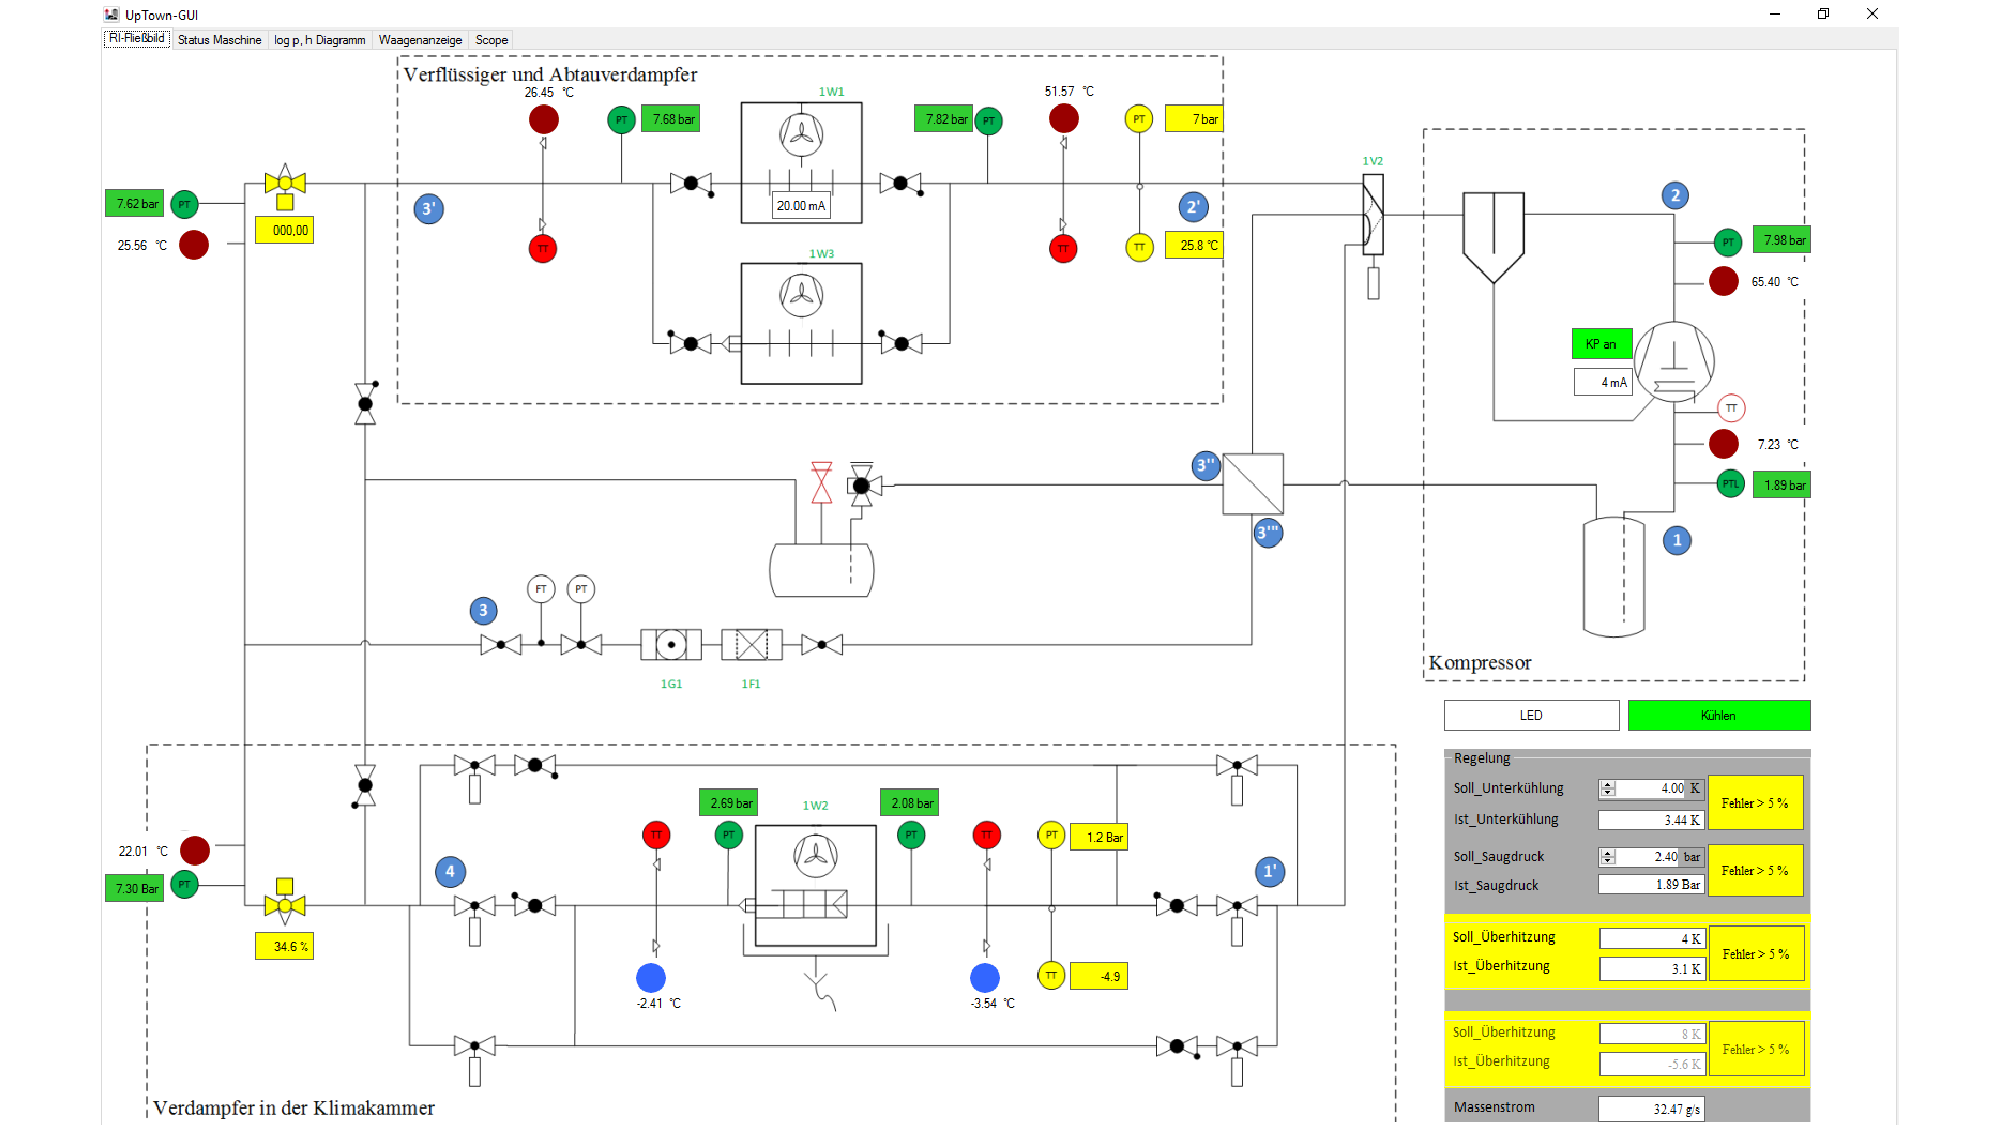
\includegraphics[page=1,width=1.05\textwidth]{Pictures/Versuchsaufbau/GUI.pdf}
\caption{RI-Fließbild in der GUI}
\label{fig:RI}
\end{figure}

Der erste Reiter der GUI ist das RI-Fließbild mit allen angeschlossenen Sensoren. Es gibt dem Benutzer einen Überblick über den Maschinenzustand der Anlage. Alle Temperatursensoren haben neben ihrer Dezimalanzeige einen roten, über 0 °C, bzw. blauen,unter 0 °C, Punkt. Die Drucksensoren sind alle grün dargestellt und die Expansionsventil-Sensoren jeweils in gelb. Neben dem Kompressor steht der aktuelle Steuerstrom. Ein LED rechts neben dem Kompressor gibt an, ob das Kompressor-Schütz an oder aus ist. 
Beim Verflüssiger wird ebenfalls der aktuelle Steuerstrom angezeigt. 

Unten rechts im Reiter stehen die Istwerte und die Sollwerte der PID-Regler. Die Sollwerte lassen sich verändern. Der Soll-Unterkühlungswert der Expansionsventile lassen sich nicht per SPS einstellen. Änderungen für einen Parameter in den Einstellungen oder Sollwert-Änderung, deswegen müssen jegliche Änderungen am Expansionsdisplay händisch durchgeführt werden. Ist der Fehler eines PID-Regler kleiner als 5 $\%$ Abweichung, so wird das LED grün.     


\subsubsection*{Uptown: Steuerung über Statusmaschine}

\begin{figure}[htb]
\centering		\includegraphics[page=2,width=1.05\textwidth]{Pictures/Versuchsaufbau/GUI.pdf}
\caption{RI-Fließbild-Reiter in der GUI}
\label{fig:RI}
\end{figure}

Auf der zweiten Seite der GUI ist die Steuerung abgebildet. Hier lässt sich die KA starten, steuern und ausschalten. Links in der grauen Box sind die Transitionsvariablen für die Bedienung der Statusmaschine angebracht. 

Die KA verfügt über einen \textit{Automatik-Modus}. Für den Automatikmodus muss eine Vereisungszeit und eine Abtaumethode ausgewählt werden. Die Statusmaschine führt dann die Transitionen zwischen Vereisung und Abtauen automatisch durch. Sind die zwei Parameter eingestellt, muss nur noch \textit{Kühlen} aktiviert werden und die Statusmaschine führt die Messungen automatisch durch. 

In dem blau hinterlegtem Feld beziehen sich auf den Kühlmodus; rot hinterlegt auf den Abtaumodus. Über \textit{Kühlen} wird der Vereisungsvorgang gestartet und über \textit{Kühlen abbrechen} wieder gestoppt. Wurde \textit{Kühlen} aktiviert, so startet die KA automatisch mit dem Modus \textit{Vollautomatik}. Der \textit{Manueller Modus} ist nur für besondere Zweck in der Inbetriebnahme zu verwenden.

Über \textit{Abtauen} lässt sich ein Abtaumodus starten. Ist \textit{Abtauen} aktiviert, kann die beliebige Abtaumethode ausgewählt werden. Erst nach Auswahl der Abtaumethode startet der Abtauvorgang (vgl. \ref{subsec:Statusmaschine}: Statusmaschine: Abtauen ). Soll der Abtauvorgang abgebrochen werden, so muss \textit{Abtauen abbrechen} aktiviert werden. Im Modus \textit{elektrisch Abtauen}, kann die Heizstufe geändert werden. Die Heizstufe muss zwischen 0 und 10 V liegen. Liegt sie außerhalb, so wird automatisch das obere oder untere Limit als Heizstufe gesetzt. Bei einer Heißgas-Abtauung kann zusätzlich die \textit{Abtauzeit} eingestellt werden. Die \textit{Abtauzeit} ist bestimmt die Dauer, die das Heißgas durch den vereisten Verdampfer strömt.  

Die zwei untersten Checkfelder sind \textit{PumpDown durchführen} und \textit{PumpDown$\_$rev durchführen}. Die zwei Vorgänge dienen der Kältemittelrückführung in den Sammler. Ein bis mehrere PumpDowns sollten vor dem Anlagenstillstand durchgeführt werden, um möglichst viel Kältemittel in den Sammler zu befördern. 

In der Mitte befindet sich die Ablaufstruktur der Statusmaschine. Das Bild dient nur der gesamte Übersicht über den Prozess und dan Ablauf. Im obereren rechten Teil sind die Komponenten des Kältekreislaufes aufgelistet. Die LEDs neben den Komponenten geben Auskunft darüber, ob die Komponenten an- oder ausgeschaltet sind.   Über das Schaltfeld \textit{SPS} wird die ADS-Verbindung zur SPS hergestellt. Bei "grün" ist eine Verbindung hergestellt und bei "rot" besteht keine Verbindung. 



\subsubsection*{Uptown: Log p,h-Diagramm}

\begin{figure}[htb]
\centering		\includegraphics[page=3,width=1.05\textwidth]{Pictures/Versuchsaufbau/GUI.pdf}
\caption{log p,h-Diagmramm-Reiter in der GUI}
\label{fig:RI}
\end{figure}

Der dritte Reiter der GUI ist eine Darstellung der Zustandspunkte in einem log p,h-Diagramm. Jeder Zustandspunkt ist in einem magenta farbigen Punkt inklusive seiner Bezeichnung in dem Diagramm wiederzufinden. Die Darstellung gibt dem Benutzer sehr schnell Auskunft über den Zustand des Systems. Jeder Zustandspunkt wird jede Sekunde aktualisiert. 

Zusätzlich sind die Zustandspunkt mit ihren zugehörigen Werten von Druck, Temperatur und Enthalpie im grauen Fenster hinterlegt. Für den Kompressor, Verflüssiger und den Verdampfer gibt die letzte Spalte den bilanzierten Wärmestrom jeder Komponente in kW an. 

\subsubsection*{Uptown: Wägesystem}

\begin{figure}[htb]
\centering		\includegraphics[page=4,width=1.05\textwidth]{Pictures/Versuchsaufbau/GUI.pdf}
\caption{Wägesystem-Reiter in der GUI}
\label{fig:RI}
\end{figure}

Der Reiter des Wägesystems ist aufgeteilt in 3 Bereiche (markiert mit 1,2,3). Der erste Bereich, links, stellt den Luftkühler aus einer Vogelperspektive dar. Das ermittelte Gewicht der eingesetzten Waagen ist in unterschiedlichen Farben hinterlegt und befinden sich unter den Aufhängepunkten des Luftkühlers auf den Blattfedern. Die farblich hinterlegte Anzeige zeigt die Gewichtsanzeige nach dem "TARE"-Befehl. Die in grau hinterlegte Anzeige zeigt das tatsächliche, gemessene Gewicht der Waage. 

Der mittlere Bereich(mit 2 makiert) zeigt den Luftkühler von der Seite. Hier sind 4 Oberflächentemperaturfühler am jeweils Eingang der Wärmeübertragerpacks. Der Verdampfer besteht aus vier solcher Wärmepacks. Neben den Oberflächentemperaturfühler sind auch noch der Ein- und Ausgang des Verdampfers mit einem Temperaturfühler versehen. Unter dem Luftkühler befindet sich die fünfte Waage, die das Schmelzwasser wiegt. 

Der rechte Bereich (markiert mit 3) ist aufgeteilt in weitere Zwei Reiter:
\begin{itemize}
\item	\textit{Anleitung Kalibrierung}
\item	\textit{Messwerte}.	
\end{itemize}


Der Karteireiter \textit{Messwerte} stellt verschiedene Messkurven dar. Die Messkurven entsprechen Messprojekten aus TwinCat und werden über ein Benutzerelement in die GUI integriert. Über die Bedienflächen lassen sich Messungen starten und stoppen und falls gewünscht auch als Scope-Datei exportieren. Zurzeit sind 4 Messkurven unter \textit{Messwerte} hinterlegt:

\begin{itemize}
\item	Waagen
\item	Bereifungsmenge
\item	2D-Schwerpunkt
\item 	Ventilöffnung vom Expansionsventil
\end{itemize}

In dem Reiter Waagen-Kalibrierung wird der Benutzer durch den Waagen-Kalibrierungsprozess geleitet. Dieser besteht aus (a)Gewichts-Kalibrierung, (b)Ventilator-Kalibrierung und (c)Reset-Waagen, siehe Abbildung \ref{fig:AnleitungKalibrierung}.  Der gesamte Kalibrierungsprozess dauert 1 h, weiter Informationen siehe Abschnitt \ref{sec:Kalibrierung Wägesystem}. 


\begin{figure}[htb]
\centering		\includegraphics[width=0.40\textwidth]{Pictures/GUI/AnleitungKalibrierung.png}
\caption{Karteireiter \textit{Anleitung Kalibrierung}}
\label{fig:AnleitungKalibrierung}
\end{figure}

\subsubsection*{Uptown: Scope}

\begin{figure}[htb]
\centering		\includegraphics[page=5,width=1.05\textwidth]{Pictures/Versuchsaufbau/GUI.pdf}
\caption{Scope-Reiter in der GUI}
\label{fig:RI}
\end{figure}

Unter dem Karteireiter \textit{Scope} sind alle Komponenten des Kältekreislaufes bilanziert. Für jede Komponente ist die Ein- und Ausgangstemperatur und -druck abgebildet. Für den Luftkühler sind zusätzlich noch die 4 Oberflächentemperaturen bei den Temperaturen integriert. Nach dem die Graphen gestartet worden sind, lassen sie sich jeder Zeit per \textit{Pausen}-Symbol anhalten und per Zoomfunktion genauer untersuchen. 
Aus Lizenzgründen lassen sich Prozesse maximal eine Stunde lang mit aufzeichnen. 
Unter "Datei$\rightarrow$ Datei laden " lassen sich beliebige Scope-Measurementprojekte in den Karteireiter laden und ausführen. 

